\section{内核优化与比较}
\subsection{时空优化1——exec系统调用优化}

在前面的章节中,我们已经介绍了exec系统调用,其作用是替换当前进程的地址空间和上下文,使得该进程执行新程序。这个系统调用结合fork系统调用,可以创建新进程。大多数参赛队伍均实现了该功能,并且可以通过大赛的测试,首届大赛冠军Ultra OS便是例子。笔者进行了Ultra OS的exec系统调用分析实验,主要方法是使用exec调用10次busybox,在系统内插入采集时延的观测点,利用日志输出相应时延数据。最后得到图\ref{exam-1}的结果。

\begin{figure}[htbp]
	\centering
	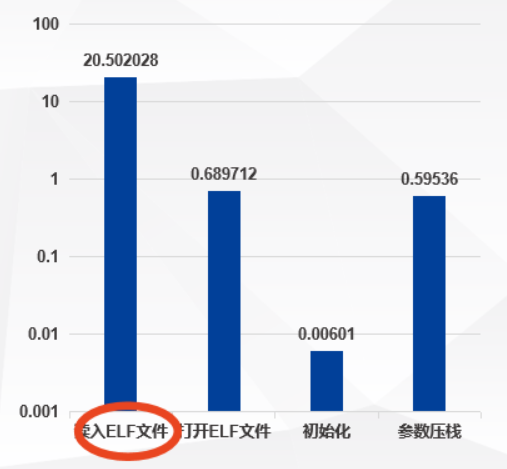
\includegraphics[scale=0.75]{figures/10-04/10-04-01.png}
	\caption{exec系统调用分析实验结果}
	\label{exam-1}
\end{figure} 

不难发现,读入ELF文件的时延占整个系统调用时长的96.45\%,已然成为exec最长的关键路径。如果不能减少该部分的时间开销,将会很大程度上影响该系统调用的性能。

笔者进一步分析Ultra OS中exec系统调用加载elf文件的过程,得到如图\ref{exam-2}的结果。

\begin{figure}[htbp]
	\centering
	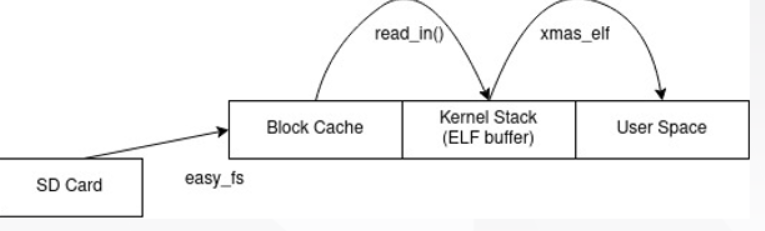
\includegraphics[scale=0.75]{figures/10-04/10-04-02.png}
	\caption{exec系统调用加载elf文件过程}
	\label{exam-2}
\end{figure}

不难发现elf文件加载时延较大的原因是复制冗余,主要体现在:
\begin{itemize}
	\item \textbf{一次调用多次复制}。 elf文件内容需要从块缓存先拷贝到内核栈中的Elf buffer,再从Elf Buffer拷贝到用户空间,无形中增大了时延。
	
	\item \textbf{重复调用多次复制}。 每次读取同一elf文件时,没有缓存,需要重新完场图 中的过程,进一步增大时延。
\end{itemize}

为了解决该问题,NPUcore使用了写时复制、elf caching、零拷贝的方法,成功降低了复制冗余的问题。在与Ultra OS的对比实验中,NPUcore的时延均显著降低。

\begin{figure}[htbp]
	\centering
	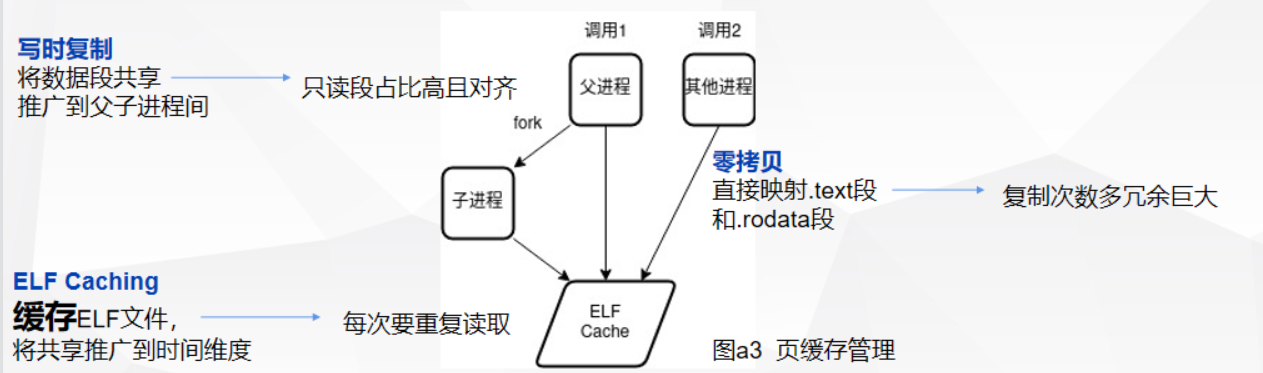
\includegraphics[scale=0.5]{figures/10-04/10-04-03.png}
	\caption{NPUcore对于exec系统调用的创新处理}
	\label{exam-3}
\end{figure}

接下来详细介绍NPUcore对于exec系统调用的优化过程,读者可以通过图\ref{exam-3}辅助理解。

\textbf{优化目标}\;由于exec系统调用的主要延迟在于冗余拷贝,NPUcore的优化目标是减少拷贝,甚至做到多次变0次Copy或者只读文件。

\textbf{优化方法}\;利用RISC-V页表共享和缺页中断的特性,可以实现“需要时”直接使用ELF Cache内的ELF文件内容,而不需要再多次或重复Copy。需要时,指多次执行同一elf文件和父进程调用folk创建子进程时。

在以上优化思想的指导下,NPUcore添加了以下功能:

\textbf{写时复制}\;考虑到只读段内容占比高且对齐,NPUcore将数据段共享推广到父子进程间。

\textbf{elf caching}\;考虑到每次使用同一个elf文件时都要重复读取,NPUcore通过实现缓存ELF文件,将共享推广到时间维度。

\textbf{零拷贝}\;考虑到.text段和.rodata段映射过程中需要多次复制且冗余较大,NPUcore在.text段和.rodata段使用的是直接映射的方式。

\begin{figure}[htbp]
	\centering
	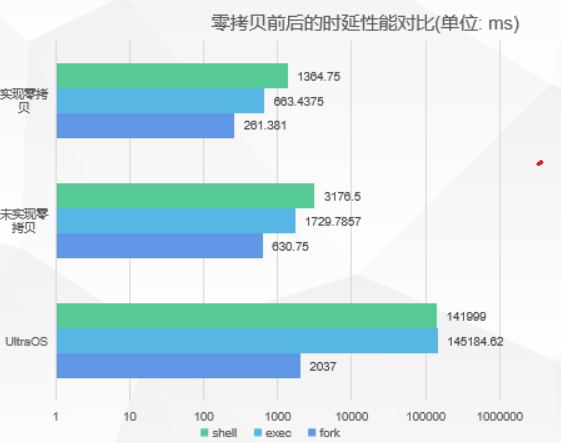
\includegraphics[scale=0.75]{figures/10-04/10-04-04.png}
	\caption{exec系统调用优化效果}
	\label{exam-4}
\end{figure}

为了检验以上优化的效果,笔者设计实验比较时延性能对比。分别设置实现零拷贝,未实现零拷贝,Ultra OS三组,分别运行shell,exec,folk三个程序,记录时延,得到图\ref{exam-4}的结果。

可以看出零拷贝的性能比不实现零拷贝的性能高出1倍还多,而Ultra OS的性能由于冗余拷贝的存在,性能远不及前两组。

\subsection{时空优化2——文件系统缓存优化}

在文件系统章节,笔者介绍过PageCache和BufferCache,这些都是文件系统块缓存的部分,目的是为了缩小持久化设备和内存的读写速度差异。

\begin{figure}[htbp]
	\centering
	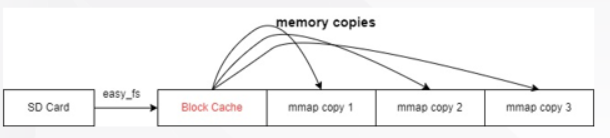
\includegraphics[scale=0.75]{figures/10-04/10-04-05.png}
	\caption{Ultra OS中的文件缓存过程}
	\label{exam-5}
\end{figure}

事实上,许多操作系统,包括清华大学的rCore以及哈工大的Ultra OS均实现了该功能。但是,以Ultral OS为例,其块缓存BlockCache设计中存在一个问题:在mmap系统调用时,多个进程调用同一个文件时,需要将文件内容分别拷贝到相应的进程空间,这就导致了多次数据拷贝的问题,造成了时延和空间上的冗余。图\ref{exam-5} 可以说明这一点。

NPUcore基于此进行优化,调整了块缓存的读写策略,从而省去了拷贝的过程,从而减少了时延和空间冗余,详细过程如下。

\textbf{优化目标} \; 减少不必要的拷贝(多次拷贝变一次拷贝)

\textbf{优化思想} \; 仍是利用RISC-V页表共享和缺页中断的特性,多个用户程序可以仅通过mmap系统调用建立的映射关系直接读写PageCache中的数据。

简而言之,就是用地址映射的方式,使得进程可以直接访问PageCache,从而省略了从PageCache拷贝数据的过程,图 解释了该过程。

\begin{figure}[htbp]
	\centering
	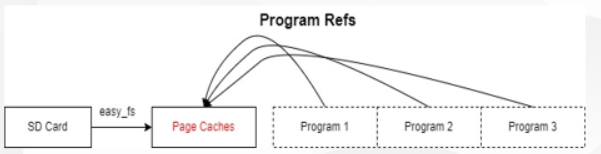
\includegraphics[scale=0.75]{figures/10-04/10-04-06.png}
	\caption{NPUcore的文件缓存过程}
	\label{exam-6}
\end{figure}

\textbf{懒分配与写时复制}\; 图\ref{exam-7} 解释了两种写入情况,写时复制和直接写入。NPUcore使用了写入复制,当进程写入数据时复制PageCache,将数据写入复制后的PageCache。

\begin{figure}[htbp]
	\centering
	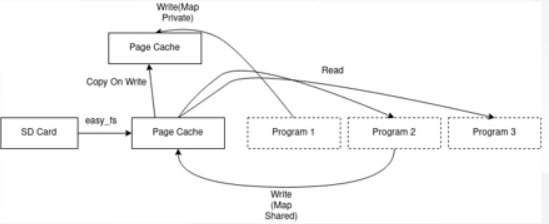
\includegraphics[scale=0.6]{figures/10-04/10-04-07.png}
	\caption{写时复制和直接写入}
	\label{exam-7}
\end{figure}

\textbf{页为单位} \; 块设备层的单位为块,而内存管理使用的单位为页。如果使用地址映射的方法访问cache则会出现单位问题,这也是为什么Ultra OS只能拷贝的原因。NPUcore这里设计了两个Cache,一个BufferCache用于缓存块设备中的数据,而PageCache实现块向页的转化。此过程可参考图\ref{exam-8}。

\begin{figure}[htbp]
	\centering
	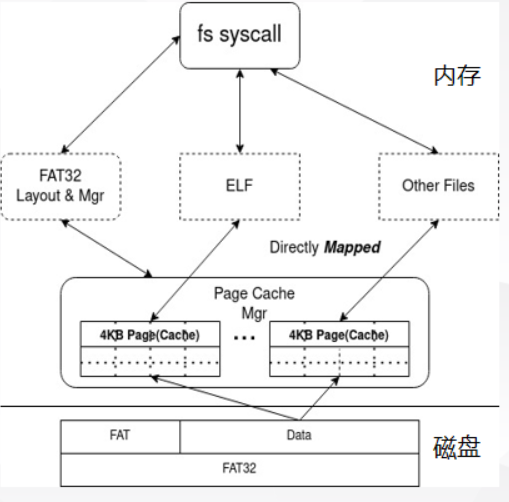
\includegraphics[scale=0.6]{figures/10-04/10-04-08.png}
	\caption{NPUcore的PageCache}
	\label{exam-8}
\end{figure}

\textbf{缓存与回收} \; 此部分与Cache相关。在文件系统中提到,整个内存地址空间均可以作为Cache的空间,所以只要空间足够就可以缓存数据,当内存已满时使用替换策略回收。

在实现了上述功能之后,笔者设计页缓存管理实验评估优化效果,分别使用旧缓存体系和新缓存体系分别测量mmap时延,分为file\_rd io\_read,file\_rd open\_to\_close和mmap_rd io\_rd.

\begin{figure}[htbp]
	\centering
	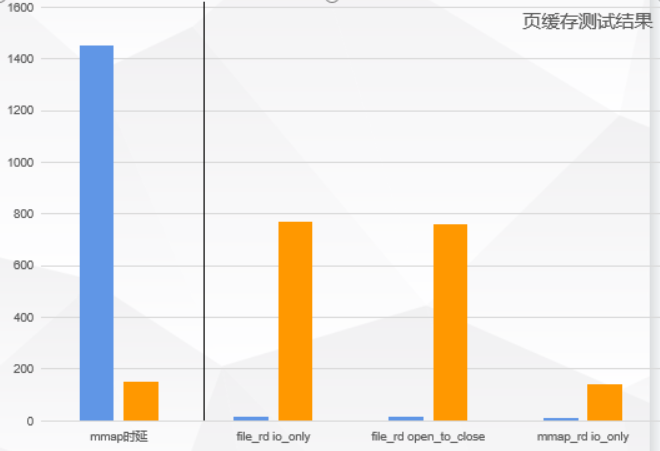
\includegraphics[scale=0.5]{figures/10-04/10-04-09.png}
	\caption{NPUcore的PageCache}
	\label{exam-9}
\end{figure}

实验结果如图\ref{exam-9}所示。从图中可以看出,mmap的时延新缓存体系与旧缓存体系相比有了较大的降低,其他部分的数据却是旧缓存体系占优。由于多了一层cache,所以其他部分延迟的增加也是在意料之中。



